\newpage
\title{LEZIONE 4 16/03/2020}\newline
[Non c'è registrazione lezione] \newline
\textbf{Update:} Trovata registrazione di backup! \textbf{link} \href{https://onedrive.live.com/?authkey=%21AATVJK3srNwxGzs&id=EE092FF4FF7B5B0E%212158&cid=EE092FF4FF7B5B0E}{clicca qui per registrazione di back up}
\section{Linearizzazione di sistemi dinamici non lineari (SD, NL, SISO, TC) nell'intorno di un equilibrio}
Consideriamo un sistema dinamico non lineare (TI):
\[
    S: \begin{cases}
        \dot{x} = f(x,u)\\
        y = g(x,u)
    \end{cases}
\]
e un suo equilibrio $(\bar{u}, \bar{x}, \bar{y})$.\newline
\newline
Volgiamo determinare un sistema dinamico lineare tempo invariante che approssimi il comportamento di $S$ nell'intorno dell'equilibrio, cioè finchè $u(t)$, $x(t)$ e $y(t)$ non si discostano "troppo" dai valori $\bar{u}$, $\bar{x}$ e $\bar{y}$ di equilibrio.
\subsection{Per l'equazione di stato}
Consideriamo \textbf{l'equazione di stato} e sviluppiamola in serie fermandoci al primo ordine:
\[
    f(\bar{x} + \delta x, \bar{u} + \delta u) = \cancel{ f(\bar{x}, \bar{u})} + f_x|_{\bar{x}, \bar{u}}\delta x + f_0|_{\bar{x}, \bar{u}} \delta u + \dots
\]
dove
\begin{itemize}
    \item $\delta x$ e $\delta u$ rappresentano gli scostamenti di $x$ e di $u$ rispetto all'equilibrio;
    \item $f(\bar{x}, \bar{u})$ vale $0$ perchè $\bar{x}$ è stato di equilibrio per $u = \bar{u}$:
    \item $f_x$ è la derivata parziale rispetto a $x$: $\frac{\delta f}{\delta x}$;
    \item $(+ ...)$ indica i termini di ordine superiore al primo dello sviluppo.
\end{itemize}
Calcoliamo ora la derivata temporale dello scostamento di $x$ rispetto all'equilibrio:
\[
    \frac{d}{dt} (\bar{x} + \delta x) = \frac{d}{dt} (\delta x) = \delta \dot{x}
\]
Siccome $\dot{x} = f(x,u)$ e $\dot{x} = \delta \dot{x}$ e $x = \bar{x} + dx$ e $u = \bar{u} + \delta u$, posso scrivere:
\[
    \delta \dot{x} = f_x|_{\bar{x}, \bar{u}} \delta x + f_u |_{\bar{x}, \bar{u}} \delta u + \dots
\]
che è un'equazione di stato lineare, alle variazioni.\newline
\newline
Abbiamo dunque trovato l'equazione di stato del sistema linearizzato.
\subsection{Per l'equazione d'uscita}
Consideriamo ora \textbf{l'equazione d'uscita} $y = g(x,u)$ e come prima sviluppiamola in serie fermandoci al primo ordine:
\[
    g(\bar{x} + \delta x , \bar{u} + \delta u) = g(\bar{x}, \bar{u}) + g_x|_{\bar{x}, \bar{u}} \delta x + g_u |_{\bar{x}, \bar{u}} \delta u + ...
\]
dove
\begin{itemize}
    \item $g(\bar{x} + \delta x , \bar{u} + \delta u) = g(x,u) = y$;
    \item $g(\bar{x}, \bar{u}) =\bar{y}$;
    \item $(+ ...)$ indica i termini di ordine superiore al primo dello sviluppo.
\end{itemize}
Per cui possiamo scrivere:
\[
    y - \bar{y} = g_x|_{\bar{x}, \bar{u}} \delta x + g_u |_{\bar{x}, \bar{u}} \delta u
\]
Da cui ricaviamo:
\[
    \delta y = g_x|_{\bar{x}, \bar{u}} \delta x + g_u |_{\bar{x}, \bar{u}} \delta u
\]
che è un'equazione d'uscita lineare.\newline
\newline
Abbiamo dunque trovato l'equazione dell'uscita del sistema linearizzato.
\subsection{Sistema linearizzato nell'intorno dell'equilibrio $\bar{u}, \bar{x}, \bar{y}$}
\[
    \mathcal{L}^\delta : \begin{cases}
        \delta \dot{x} = f_x |_{\bar{x},\bar{u}} \delta x + f_u|_{\bar{x},\bar{u}} \delta u\\
        \delta y = g_x|_{\bar{x},\bar{u}} \delta x + g_u |_{\bar{x},\bar{u}} \delta u
    \end{cases}
\]
con $ \delta u = u - \bar{u}$, $\delta x = x -\bar{x}$, $ \delta y = y - \bar{y}$.
\subsection{Interpretazione}
[immagine dagli appunti del prof]
\begin{center}
    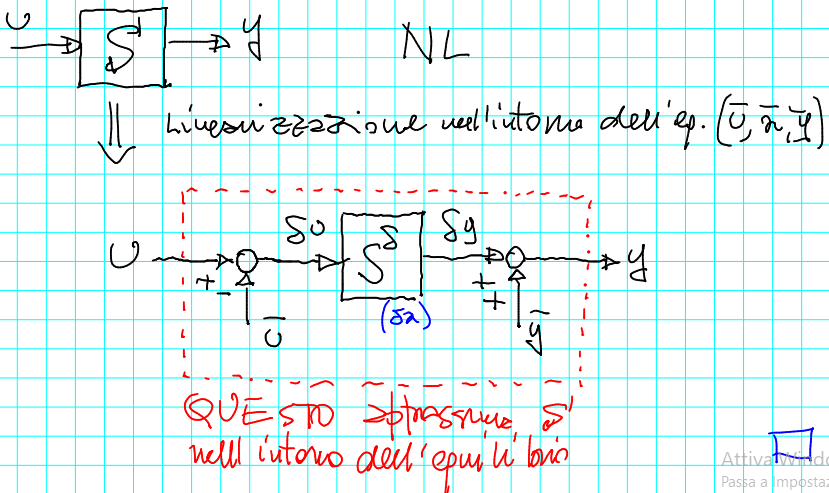
\includegraphics[height=7cm]{../lezione4/img1.PNG}
\end{center}
Facendo una linearizzazione di un sistema non lineare $S$, con un ingresso $u$ e un'uscita $y$, nell'intorno dell'equilibrio $(\bar{u}, \bar{x},\bar{y})$, otteniamo un sistema $S^\delta$ che ha come ingresso $\delta u$ e un'uscita $\delta y$, cioè l'ingresso e l'uscita sono le variazioni. Allora per avere un sistema linearizzato che abbia un effettivo ingresso $u$ e un'uscita $y$, dobbiamo aggiungere i due nodi sommatori che si vedono in figura.\newline
\newline
\textbf{oss.} Il riquadro tratteggiato di rosso nell'immagine (non solo $S^\delta$) è ciò che approssima $S$ nell'intorno dell'equilibrio, un errore molto tipico è pensare che il solo $S^\delta$ sia la linearizzazione.
\newpage
\section{Stabilità}
\subsection{Stabilità di un equilibrio}
\subsubsection{Equilibrio stabile (S)}
Sia $\bar{x}$ uno stato di equilibrio del sistema dinamico non lineare generico $\dot{x} = f(x,u)$ per $u = \bar{u}$ costante, si dice equilibrio stabile se
\[
    \;\forall\; \epsilon > 0 \;\; \exists \; \delta > 0 \;\;:\;\; ||x(0) - \bar{x}|| < \delta \Rightarrow  ||x(t) - \bar{x}|| < \epsilon \;\;\;\forall\;t \geq 0
\]
dove per $|| \dots ||$ si intende la "norma" (lunghezza del vettore).\newline
\newline
Questo significa che desideriamo che il sistema, partendo vicino all'equilibrio, non si allontani mai dall'equilibrio più di un $\epsilon$, allora qualunque sia questo $\epsilon$ scelto, se l'equilibrio è stabile, esiste un $\delta$ tale per cui se "partiamo" non più lontani di $\delta$ dall'equilibrio, allora tutto il movimento rimarrà vicino all'equilibrio entro $\epsilon$.\newline
\newline
Interpretazione con $x$ scalare:\newline
[immagine dagli appunti del prof]
\begin{center}
    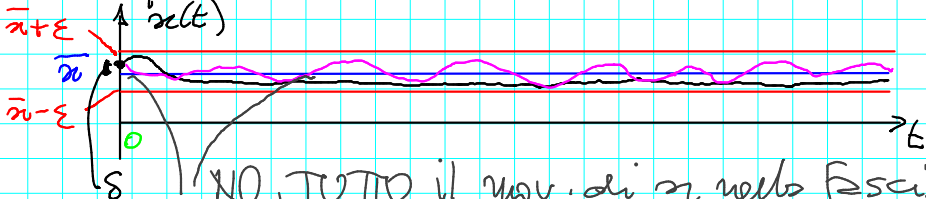
\includegraphics[height=3cm]{../lezione4/img2.PNG}
\end{center}
Prendiamo un valore di equilibrio $\bar{x}$ (in blu), allora tutto il movimento si deve sviluppare in una fascia compresa fra $\bar{x}+ \epsilon$ e $\bar{x} - \epsilon$. Qualunque sia questo $\epsilon$ preso, esiste un $\delta$, tale per cui, partendo dal valore $x(0) = \bar{x}+ \delta$, l'intero movimento si sviluppa all'interno della fascia.\newline
Due esempi di movimento in stabilità sono la curva nera e la curva rosa. Un esempio non valido di stabilità è la curva grigia, esce dalla fascia rossa!
\subsubsection{Equilibrio asintoticamente stabile (AS)}
Si dice asintoticamente stabile l'equilibrio per cui, oltre a valere la stabilità semplice stabile, vale
\[
    ||x(t) - \bar{x}|| \rightarrow 0  \;per \; t \rightarrow \infty
\]
Cioè il movimento oltre a essere contenuto nella fascia compresa fra $\bar{x}+ \epsilon$ e $\bar{x} - \epsilon$, deve ritornare esattamente al punto di equilibrio $\bar{x}$.
\subsubsection{Equilibrio instabile (I)}
In tutti gli altri casi.
\subsection{Stabilità nei sistemi dinamici (SD) lineari tempo invarianti (LTI)}
\subsubsection{Stabilità come proprietà di sistema (SD LTI a TC)}
L'equazione di stato per sistemi dinamici lineari tempo invarianti a tempo continuo è:
\[
    \dot{x} = Ax + bu
\]
Sia $\bar{x}$ uno stato di equilibrio per $u = \bar{u}$, allora, prendendo lo stato iniziale all'equilibrio e mantenendo l'ingresso al valore $\bar{u}$ lo stato non si muove e rimane nell'equilibrio:
\[
    \begin{rcases}
        x(0) &= \bar{x}\\
        u(t) &= \bar{u} \;\;\; t\geq 0
    \end{rcases} \rightarrow  x(t) = \bar{x} \;\;\;t \geq 0
\]
Quindi possiamo ora esprimere il movimento $x(t)$ con la formula di Lagrange e porlo uguale a $\bar{x}$
\[
    x(t) = e^{At} \bar{x} + \int_{0}^{t}e^{A(t-\tau)} b \bar{u} d \tau = \bar{x}
\]
\ \newline 
Vediamo ora cosa succede se invece di partire dallo stato di equilibrio ci scosiamo di un certo valore $\Delta \bar{x}$. Consideriamo il \textbf{movimento perturbato} $x_{\Delta}$, prodotto da $u(t) = \bar{u}$ e $x(0) = \bar{x} + \Delta \bar{x}$
\[
    x_{\Delta}(t) = e^{At}(\bar{x} + \Delta \bar{x}) + \int_{0}^{t}e^{A(t- \tau)}b \bar{u} d \tau
\]
in cui notiamo che il secondo termine $\int_{0}^{t}e^{A(t- \tau)}b \bar{u} d \tau$ è uguale a prima.\newline
\newline
Scriviamo la differenza fra il movimento perturbato appena scritto e $\bar{x}$ trovato prima:
\[
    x_\Delta (t) - \bar{x} = e^{At} \Delta \bar{x}
\]
Notiamo che gli integrali si sono elisi a vicenda.\newline
\newline
Da quest'ultima equazione, deduciamo diverse osservazioni:\newline
\newline
\textbf{oss.} Questa equazione ci mostra che la maniera in cui $x_\Delta$ di muove rispetto a $\bar{x}$ (cioè il termine $x_\Delta (t) - \bar{x}$) non dipende dal particolare $\bar{x}$ (che al secondo membro dell'equazione non compare).\newline
\newline
\textbf{oss.}  Tutti gli equilibri (se ve ne sono) hanno le stesse caratteristiche di stabilità.\newline
Quindi \textbf{nei sistemi lineari} (tempo invarianti) \textbf{la stabilità è una proprietà del sistema}, e non una proprietà dell'equilibrio, \textbf{non ci possono essere equilibri instabili e equilibri stabili in uno stesso sitema lineare, devono essere tutti dello stesso "tipo"}. Se il sistema fosse non lineare questo discorso non varrebbe.\newline
\newline
\textbf{oss.} \textbf{La stabilità del sistema dipende soltanto dal comportamento di $e^{At}$, cioè dalla matrice $A$}.\newline
\newline
Quindi riassumendo:
\[
    x_{\Delta}(t) - \bar{x} = e^{At}\Delta \bar{x}
\]
\begin{itemize}
    \item \textbf{ Se $e^{At} \rightarrow$ tende a diventare la matrice nulla $0_{nxn}$ per $t \rightarrow  \infty$ $\Longrightarrow$ allora il sistema è AS (cioè il movimento libero di $x$ tende a $0$)};
    \item \textbf{Se $e^{At}$ diverge per $t \rightarrow  \infty$ $\Longrightarrow$ Allora il sistema è I (perchè il movimento libero di $x$ diverge, salvo eccezzioni, quali per esempio partire dall'equilibrio stesso)};
    \item \textbf{Se $e^{At}$ nè tende a $0$ nè diverge per $t \rightarrow  \infty$ $\Longrightarrow$  Allora il sistema è S}.
\end{itemize}
\ \newline
\textbf{es.}  Sistema LTI a TC di ordine 1:\newline
$\dot{x} = a x$, con $a$ scalare e equilibrio $\bar{x} = 0$.\newline
$x(0) = \Delta \bar{x}$\newline
\[
    x(t) = e^{at} \Delta \bar{x}\Rightarrow \begin{cases}
        a < 0 \;\;\;\; & x(t) \rightarrow  0 = \bar{x} \;\text{equilibrio AS}\;\\
        a = 0 \;\;\;\; & x(t) = \Delta \bar{x} \;\text{equilibrio S}\;\\
        a > 0 \;\;\;\; & x(t) \;\text{diverge}\;\;\;\text{equilibrio I}\;
    \end{cases}
\]
\rule{\textwidth}{0,4pt}
\subsubsection{Proprietà di sistemi asintoticamente stabili (SD LTI a TC)}
Per i nostri scopi ci interessa principalmente la stabilità asintotica, che ha le seguenti particolari proprietà:
\begin{itemize}
    \item i movimenti liberi di $x$ e di $y$ tendono a $0$ per $t \rightarrow  \infty$, quindi tali sistemi "dimenticano lo stato iniziale", cioè da un certo punto in poi il movimento libero diventa trascurabile;
    \item Se $
        u(t) = \begin{cases}
            \text{qualsiasi segnale}\; \;\; & t< \bar{t}\\
            0 & t \geq \bar{t}
        \end{cases}$ allora per $t \geq \bar{t}$ c'è solo movimento libero e quindi $x,y \rightarrow 0$ per $t \rightarrow \infty$.
\end{itemize}
\subsubsection{Matrice A e Stabilità (SD LTI a TC e a TD)}
\subsubsection*{caso a tempo continuo (TC) e A diagonalizzabile}
Caso in cui $A$ è diagonalizzabile.\newline
\newline
Partiamo dal movimento libero di $x$: $x_L (t) = e^{At} x(0) = e^{T diag\{\lambda_i\}T^{-1} t}x(0) = T diag\{e^{\lambda_i t}\}T^{-1}x(0)$, dove $x_L(t)$ è il movimento libero di $x$, T è la matrice che diagonalizza $A$ e i vari $e^{\lambda_it}$ prendono il nome di \textbf{modi del sistema}.\newline
\newline
Se $A$ è reale, allora $\lambda_i$ sono o reali o coppie complesse coniugate.\newline
\newline
Se il movimento libero tende a $0$ per ogni $x(0)$ vuol dire che tutti i modi devono tendere a $0$ per $t \rightarrow \infty$.
\begin{itemize}
    \item se $\lambda_i$ è reale, allora si definiscono
    \[
        \begin{cases}
            \lambda_i >0 \;\;& \text{modo divergente}\;\\
            \lambda_i =0 \;\;& \text{modo costante}\;\\
            \lambda_i <0 \;\;& \text{modo}\;\rightarrow  0
        \end{cases}
    \]
    \item se $\lambda_{h,k} = \alpha \pm i \beta$ è una coppia complessa coniugata, con $\alpha$ e $\beta$ reali, allora si ha che $e^{(\alpha + i \beta)t} = e^{\alpha t} \cancel{sin(\beta t) + i cos(\beta t)}$ [perchè $sin(\beta t) + i cos(\beta t)$ è limitata] e quindi si definiscono
    \[
        \begin{cases}
            Re(\lambda) < 0 \;\; & \text{modo convergente}\;\\
            Re(\lambda) = 0 \;\; & \text{modo limitato ma non tendente a $0$}\;\\
            Re(\lambda) > 0 \;\; & \text{modo divergente}\;
        \end{cases}
    \]
\end{itemize}
Notiamo che tutto ciò che conta ("in entrambi i casi") è la parte reale degli autovalori.\newline
\newline
Possiamo quindi dedurre dei \textbf{criteri di stabilità basati sull'analisi degli autovalori di $A$}:
\begin{itemize}
    \item Tutti gli autovalori di $A$ hanno $Re <0$ $\Longleftrightarrow$ Sistema AS.
    \item Almeno un autovalore di $A$ ha $Re > 0$ $\Longrightarrow$ Sistema I.
    \item Tutti gli autovalori di $A$ hanno $Re \leq 0$ e ne esiste almeno uno con $Re = 0$ $\Longrightarrow$ $\begin{cases}
        \text{sistema I;}\;\\
        \text{oppure sistema S, ma non AS.}\;
    \end{cases}$. \newline
    Per capire se si tratta di un sistema stabile o instabile bisogna andare a calcolare il movimento libero per un generico ingresso $x(0)$ e vederne il comportamento per $t \rightarrow \infty$. Se il movimento libero rimane sempre limitato allora il sistema è stabile, se il movimento libero diverge (anche una sola delle componenti del movimento libero) allora il sistema è instabile (Puoi trovare degli esempi di esercizi nell'esercitazione $1$, es. 2 e es. 3). \newline
    Esiste anche un altro metodo (per capire meglio questo esempio guardare l'esercitazione 2 es. 9) per capire se il sistema è stabile o instabile: guardando la matrice di Jordan, se il più grande miniblocco di Jordan ha dimensione $1$ allora il sistema è stabile, altrimenti è instabile. Un buon metodo per ricordarlo è usare i seguenti due esempi che abbiamo visto a esercitazione:
    \[
        \left[\begin{matrix}
            0 & 0 \\
            0 & 0
        \end{matrix}\right] \;\;\text{ha due miniblocchi di dimensione 1 e quindi è semplicemente stabile}\;
    \]
    \[
        \left[\begin{matrix}
            0&1\\
            0&0
        \end{matrix}\right] \;\; \text{ha un miniblocco di dimensione 2 e quindi è instabile}\;
    \]
\end{itemize}

\ \newline
Noi saremo prevalentemente interessati a sistemi asintoticamente stabili, per cui è importante che tutti gli autovalori di $A$ abbiano parte reale negativa.
\subsubsection*{caso a tempo discreto (TD) e A diagonalizzabile}
Partiamo anche qua dal movimento libero: $x_L(k) = A^k x(0)$\newline
\newline
In cui $A^k = (T diag\{\lambda_i\} T^{-1})^k = T diag\{\lambda_i\}\cancel{T^{-1}T} diag\{\lambda_i\} T^{-1} \dots$ (k volte) $= T diag\{\lambda_i^k\}T^{-1}$, dove $\lambda_i^{k}$ sono i \textbf{modi del sistema}.\newline
\newline
Quindi il discorso è del tutto analogo a quello del caso a tempo continuo, solo che non conta la parte reale, ma il modulo. \textbf{Criteri di stabilità basati sull'analisi degli autovalori di $A$}:
\begin{itemize}
    \item Tutti gli autovalori di $A$ hanno $|\lambda_i| < 1$ $\Longleftrightarrow$ sistema AS.
    \item Almeno un autovalore di $A$ con modulo $|\lambda_i| > 1$ $\Longrightarrow$ sistema I.
    \item Tutti gli autovalori di $A$ hanno $|\lambda_i| \leq 1$ e ne esiste almeno uno tale che $|\lambda_1| = 1$ $\Longrightarrow$ $\begin{cases}
        \text{sistema I;}\;\\
        \text{oppure sistema S, ma non AS.}\;
    \end{cases}$. \newline
    Per capire se il sistema è instabile o stabile nell'ultimo punto, controlla l'osservazione fatta per il caso a tempo continuo.
\end{itemize}
\ \newline
\textbf{oss.} Errore tipico: Nel caso a tempo continuo si guarda la parte reale degli autovalori, nel caso a tempo discreto si guarda il modulo (!) degli autovalori.\newline
\newline
\textbf{oss.} Errore tipico: Più avanti vedremo il criterio di Routh, ma da notare è che non vale per i sistemi a tempo discreto, vale solo per sistemi a tempo continuo (!).
\subsubsection{Criteri di stabilità dedotti dalla matrice A (SD LTI a TC)}
Domanda: dato il sistema $S$ di matrice $A$, posso dire se tutti gli autovalori di $A$ hanno o meno $Re <0$ senza calcolarli, in modo da stabilire che il sistema è asintoticamente stabile??\newline
\newline
Sì, vi sono criteri per dirlo basati sull'ispezione di $A$ o del suo polinomio caratteristico $\Pi(s) = det (sI-A)$:
\begin{itemize}
    \item Siccome $det(A) = \Pi_{i=1}^{n}S_i$, dove con $S_i$ si intendono gli autovalori $\Longrightarrow$ allora se $det(A) = 0$ esiste $S_i = 0$ $\Longrightarrow$ sistema non AS.
    \item Siccome $tr(A) = \sum_{i=1}^{n}S_i$, dove con $S_i$ si intendono gli autovalori $\Longrightarrow$ se $tr(A) >0$ esiste $S_i$ tale che $Re(S_i) > 0$ $\Longrightarrow$ sistema I.
    \item Se $Re(S_i)<0$ per ogni $i$ (cioè se il sistema è asintoticamente stabile), allora i coefficienti di $\Pi(S)$ sono tutti concordi e non nulli \newline
    \textbf{oss.} Errore tipico: il viceversa vale solo per polinomi del secondo ordine.
\end{itemize}
\textbf{oss.}  Questi tre criteri non ci permettono di capire se un sistema è asintoticamente stabile, ma ci permettono facilmente di capire se non lo è (primi due criteri).\newline
\newline
\textbf{oss.} Per stabilire se un sistema è asintoticamente stabile abbiamo due possibilità: per prima cosa con i primi due dei tre criteri appena esposti stabiliamo se non è asintoticamente stabile, altrimenti, se non abbiamo avuto fortuna con questi criteri, usiamo il criterio di Routh (prossimo argomento, vedi più avanti). Un caso particolare è rappresentato dai polinomi di secondo ordine, in cui possiamo evitare di usare Routh e usare il terzo criterio appena visto.